\section{Manifolds that carry the super-loop}
\label{sec:manifolds}

The super-loop is itself a manifold, and it acts on others. Figure~\ref{fig:manifolds} collects the
manifolds that we identify; each statement is a machine check.

\emph{The $7+1$ Minkowski space.} The Hermitian bi-octonions, $\mathbf x^\dagger=\mathbf x$, are the
elements $\mathbf x=x^0_{\rm LL}\mathbf e_0+i\sum_{p=1}^7x^p_{\rm LL}\mathbf e_p$ with real coordinates
$x^p_{\rm LL}$. On them the norm is real,
\begin{equation}
N_{\rm LL}(\mathbf x)=(x^0_{\rm LL})^2-\textstyle\sum_{p=1}^7(x^p_{\rm LL})^2 ,
\label{eq:r17}
\end{equation}
with one positive and seven negative signs: they form the Minkowski space $\mathbb R^{1,7}_{\rm LL}$
of $7+1$ dimensions (N-1). The Hermitian bi-quaternions ($p\le3$) form the Minkowski space $\mathbb
R^{1,3}_{\rm LL}$ of $3+1$ dimensions, on which $SL(2,\mathbb C)$ acts by $\mathbf x\mapsto\mathbf
g\mathbf x\mathbf g^\dagger$: the familiar action of the Lorentz group on four-vectors. The
conjugations $\mathbf x\mapsto\mathbf g\mathbf x\mathbf g^\dagger$ of $\mathbb R^{1,7}_{\rm LL}$ by the
one-parameter families $\mathbf g=\exp(\theta_{\rm LL}\mathbf e_p)$ (rotations) and $\mathbf
g=\exp(\theta_{\rm LL}i\mathbf e_p)$ (boosts) of loop elements, $p=1,\dots,7$, have the generators
$\mathbf x\mapsto[\mathbf e_p,\mathbf x]$ and $\mathbf x\mapsto i(\mathbf e_p\mathbf x+\mathbf x\mathbf
e_p)$; they preserve Eq.~(\ref{eq:r17}), and the Lie algebra they generate is all of $\mathfrak{so}(1,7)$,
of dimension 28 (N-4). (The products are unambiguous: by Artin's theorem the subalgebra generated by
$\mathbf e_p$ and $\mathbf x$ is associative.)

\emph{Conjugation by the loop is not a group action.} Restricted to the loop's own Lorentz subgroup
($p=1,2,3$), the six generators preserve $\mathbb R^{1,3}_{\rm LL}$ and act on it as
$\mathfrak{so}(3,1)$, but on $\mathbb R^{1,7}_{\rm LL}$ they generate a Lie algebra of dimension
$9=6+3$ (N-5): on the four directions $i\mathbf e_4,\dots,i\mathbf e_7$ the boosts act trivially and the
rotations by the twisted action of Eq.~(\ref{eq:twist}), and the commutators separate an extra
$\mathfrak{so}(3)$ that acts on these directions alone. A group action would give back a Lie algebra of
dimension 6. This is the geometric face of the twist charge.

\emph{The $4+4$ manifold.} The real subspace $\mathbb O^{\rm s}_{\rm LL}=\mathbb H+(i\mathbb H)\mathbf
e_4$ of $\mathbb B_{\rm LL}$ is closed under the product, and the map from the split Cayley-Dickson
algebra (pairs of real quaternions with the sign $+1$ in place of the $-1$ of Eq.~(\ref{eq:cd})) that
sends the pair $(\mathbf a,\mathbf b)$ to $\mathbf a+(i\mathbf b)\mathbf e_4$ is an isomorphism onto it
(N-2): $\mathbb O^{\rm s}_{\rm LL}$ is the algebra of \emph{split octonions}, and the norm has on it the
signature $(4,4)$. Its unit elements form the pseudo-sphere $S^{3,4}_{\rm LL}$, a Moufang loop and the
$4+4$ real form of the super-loop. Inside its imaginary part, $\mathbf e_1$, $i\mathbf e_4$ and
$i\mathbf e_5$ span the Lie algebra $\mathfrak{sl}(2,\mathbb R)=\mathfrak{so}(2,1)$ (Killing form: two
positive, one negative; N-9): on the real $4+4$ manifold the Lorentz part of the super-loop is the
Lorentz group of $2+1$ dimensions, $SL(2,\mathbb R)=Spin(2,1)$, and $SO(3,1)$ needs the complex form.
The space of spinor charges is a second $4+4$ space: $\mathrm{Re}\,N_{\rm LL}$ and $\mathrm{Im}\,N_{\rm
LL}$ are, on $\mathfrak s_{\rm LL}$, two quadratic forms of signature $(4,4)$, both invariant under the
automorphisms~(\ref{eq:aut}) (N-3).

\emph{The super-loop manifold.} $\mathbb L_{\rm LL}$, Eq.~(\ref{eq:loop}), is a complex quadric of real
dimension 14; as a homogeneous space it is $Spin(7,\mathbb C)/\mathrm G_2(\mathbb C)$. It is
\emph{parallelizable}: the vector fields $X^{\rm LL}_{\mathbf x}(\mathbf w)=\mathbf w\mathbf x$ for the 14
real imaginary directions $\mathbf x$ are tangent to it, $N_{\rm LL}(\mathbf w,\mathbf w\mathbf x)=0$, and
form a frame at every point. Their Lie brackets are
\begin{equation}
[X^{\rm LL}_{\mathbf x},X^{\rm LL}_{\mathbf y}](\mathbf w)=\mathbf w[\mathbf x,\mathbf y]+2[\mathbf w,\mathbf x,\mathbf y]
\label{eq:frames}
\end{equation}
(N-7; it follows from $(\mathbf w\mathbf x)\mathbf y-(\mathbf w\mathbf y)\mathbf x$ and alternativity).
At the identity this is the Malcev bracket; elsewhere the associator makes the structure functions
depend on the point. On a Lie group the frame fields of the group's own multiplication have constant
structure functions: $\mathbb L_{\rm LL}$ is a parallelizable manifold that carries no Lie group
structure compatible with its product. Its compact real form, the unit octonions, is the seven-sphere
$S^7_{\rm LL}$; the products $L^{\rm LL}_{\mathbf e_p}L^{\rm LL}_{\mathbf e_{p'}}$ ($p<p'$) span
$\mathfrak{spin}(7)$, of dimension 21, whose stabilizer of $\mathbf e_0$ is $\mathfrak g_2$ (14), so that
$S^7_{\rm LL}=Spin(7)/\mathrm G_2$ (N-8)~\cite{Baez2002}.

\emph{The linear action closes into Lie groups.} The left multiplications by the imaginary
bi-octonions generate $\mathfrak{so}(8,\mathbb C)$ (real dimension 56), those by the imaginary octonions
$\mathfrak{so}(8)$, and those by the imaginary split octonions on $\mathbb O^{\rm s}_{\rm LL}$
$\mathfrak{so}(4,4)$ (N-6). Any \emph{linear} action of the loop on a vector space generates a Lie
group, in agreement with Theorem R; the non-associative structure lives in the product of the loop,
not in its linear action. Section~\ref{sec:renorm} uses this fact.

\begin{figure}[t]
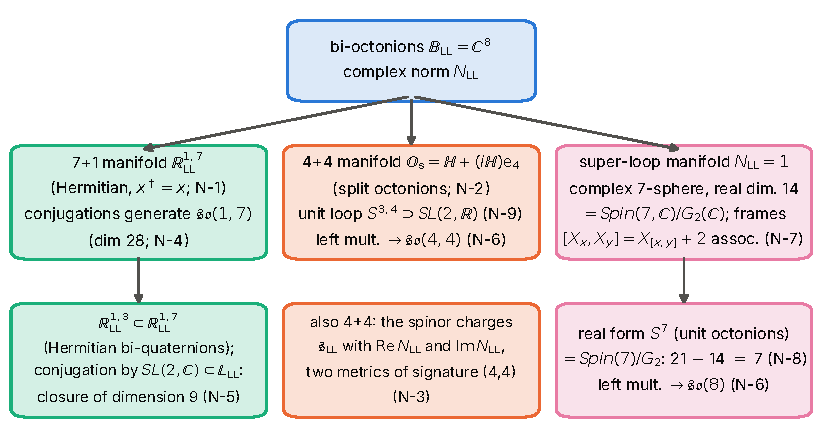
\includegraphics[width=\columnwidth]{../figures/fig_sl_manifolds.pdf}
\caption{The manifolds that carry the super-loop: $\mathbb R^{1,7}_{\rm LL}$ and $\mathbb R^{1,3}_{\rm
LL}$ (conjugation), the split octonions $\mathbb O^{\rm s}_{\rm LL}$ ($4+4$), the space of spinor charges
with its two $(4,4)$ forms, the super-loop manifold and its compact real form $S^7_{\rm LL}$. The
labels are those of the checks.}
\label{fig:manifolds}
\end{figure}
